\documentclass[11pt, a4paper]{report}
\usepackage[lmargin=2cm,rmargin=2cm,top=1.5cm,
bottom=2cm]{geometry}
\usepackage[T1]{fontenc}
\usepackage[utf8x]{inputenc} %Ha sido cambiado agregando "x" por que no aceptaba °
\usepackage[spanish,es-tabla]{babel}
\parindent=0cm
\usepackage{amsmath}
\usepackage{amssymb,amsfonts,latexsym,cancel}
\usepackage{array}
\usepackage{bm}
\usepackage{float}
\usepackage{fancyhdr}
\usepackage{graphicx}
\usepackage{epstopdf}
\usepackage[colorlinks = true,
            linkcolor = black,
            citecolor = black,
            urlcolor = blue]{hyperref}
\usepackage{longtable}
\setcounter{MaxMatrixCols}{40}
\usepackage{multicol}
\usepackage{subfigure}
\usepackage{titling}
\usepackage{titlesec}
\newcolumntype{E}{>{$}c<{$}}
\usepackage{apacite}
%\setlength{\parskip}{1em}
\raggedright % alineado a la izquierda

% oculta el texto de "Capitulo" 
%\titleformat{\chapter}[display]
%{\normalfont\bfseries}{}{0pt}{\Large}
\usepackage{pdfpages} % para insertar pdfs(anexos)

\renewcommand{\thechapter}{\Roman{chapter}}
\usepackage{pdflscape}
\usepackage{longtable}

\begin{document}
\doublespacing
\def\thesistitle{Implementación de un modelo matemático para la planificación de un viaje personalizado basado en optimización multiobjetivo para los turistas en la región Puno} % variable
\begin{center}
\vspace*{\baselineskip}

{
\bf\fontsize{19}{0}{\selectfont{UNIVERSIDAD PERUANA UNIÓN}}\\[0.5cm]

\bf\fontsize{14}{0}{FACULTAD DE INGENIERÍA Y ARQUITECTURA}\\[0.5cm]

\bf\fontsize{14}{0}{Escuela Profesional de Ingeniería de Sistemas}\\[0.5cm]
}

\vspace*{\baselineskip}

\includegraphics[scale=0.7]{Figuras/upeu}
\vspace*{2\baselineskip}

{
\fontsize{14}{0}
{\selectfont{Modelo inteligente para ayudar en la planificación de viajes personalizados para los turistas en la región Puno}}
\\[1cm]
}


{
\fontsize{14}{0}
{\bf\selectfont{Por:}}\\[0.5cm]
{\selectfont{Yuselenin Anquise Jihuaña}}\\[1cm]
{\bf\selectfont{Asesor:}}\\[0.5cm]
{\selectfont{Dr. Jorge Alejandro Sánchez Garcés}}\\[1cm]
{\bf\selectfont{Co-asesora:}}\\[0.5cm]
{\selectfont{Dra. Nelida Gladys Maquera Sosa}}\\[2.5cm]
}
\bf\fontsize{12}{0}{Juliaca,\today}

\thispagestyle{empty}
\end{center}
\pagenumbering{roman}

%\chapter*{Dedicatoria}
Dedicatoria
%\chapter*{Agradecimientos}
Agradecimientos
\renewcommand{\contentsname}{Tabla de contenidos}
\let\origaddvspace\addvspace % quita los espacios de capítulos en la lista de tablas y figuras. segun https://tex.stackexchange.com/questions/121879/remove-spacing-between-per-chapter-figures-in-lof
 \renewcommand{\addvspace}[1]{}
\tableofcontents
\clearpage
\listoftables
\clearpage
\listoffigures
\clearpage
\renewcommand{\addvspace}[1]{\origaddvspace{#1}}

\pagenumbering{arabic}
\chapter{I. DATOS GENERALES}
\section{Código}
201322747
\section{Título}
Modelo inteligente para ayudar en la planificación de viajes personalizados para los turistas en la región Puno.
\section{Línea de investigación}
Tecnología de información e innovación tecnológica.
\section{Autor del proyecto}
Yuselenin Anquise Jihuaña
\section{Fecha de presentación del proyecto}
...
\section{Firma del autor}
{
\vspace{8em}
\centering
\rule[1em]{20em}{0.5pt} % Línea para la firma
\textsc{Firma}
}
\section{Nombre del asesor}
Dr. Jorge Alejandro Sánchez Garcés
\section{Nombre del co-asesor(a)}
Dra. Nelida Gladys Maquera Sosa

\chapter{II. IDENTIFICACIÓN DEL PROBLEMA }
\chapter{III.BASES TEÓRICAS DE LA INVESTIGACIÓN}
\chapter{MATERIALES Y MÉTODOS}
\section{Descripción del lugar de ejecución}
"La Región Puno tiene una historia grandiosa de origen, de culturas pre-incas: Pukara, Tiahuanaco, Lupaca entre otros, Inca, cuyas manifestaciones aún se mantienen vivas, muchas ubicadas alrededor del Lago Titicaca, contamos con productos como la quinua, papa, alpaca entre otros, que son un aporte a la humanidad, los majestuosos paisajes que ofrece el Lago Titicaca hasta las magníficas vistas de Macusani, Carabaya, con arte rupestre y aguas termales, y la inmensa biodiversidad de la selva Puneña; somos la quinta región más grande del país, con una extensión de 71,999 Km2, y la cuarta región más poblada con 1’268,441 habitantes, la arquitectura colonial manifestada en Templos, casonas, balcones que datan del siglo XVI en Lampa, Juli, Puno, atractivos que hacen que la región tenga un potencial turístico de nivel internacional." \cite{2011PlanPERTUR}
% TODO: Se podría actualizar los datos(habitantes)

\subsection{Ubicación geográfica y límites}
"La región Puno es de gran importancia para el turismo, tiene importantes atractivos turísticos de carácter natural (Lago Titicaca, Lagunas, ríos, ceja de selva, flora, fauna, etc.), cultural (sitios arqueológicos, templos coloniales), rico y variado folklore (conocida como la Capital del Folklore Peruano).

Puno, tiene ubicación geopolítica estratégica en el continente, y una ubicación estratégica en el corredor turístico Cusco – Puno - La paz (Bolivia); con el Cusco como la gran atracción turística con el Santuario de Machu Picchu(maravilla cultural del mundo moderno), así como con las Regiónes Arequipa y Tacna, esta última con gran afluencia de turistas chilenos. Y la carretera interoceánica sur que conecta a la Región de Puno a través de Madre de Dios con el Brasil, lo que permitirá la afluencia de turistas brasileros." \cite{2011PlanPERTUR}

\subsection{Estructura poblacional}
"La base física de la región está conformada por dos zonas bien definidas: Altiplano y selva, la primera es plana y la segunda zona corresponde a la vertiente oriental de los Andes, en el altiplano peruano entre los 3,812 a 5,500 m.s.n.m, en la ceja de selva y selva alta entre los 4,200 a 500 m.s.n.m. Tiene una extensión de 71,999 Km2, que incluye 14.50 km2 de área insular lacustre y 4,996.28 Km2 de lago perteneciente al lado peruano, su población alcanza a 1’268,441 habitantes, con una densidad poblacional de 17.62 hab/km2, cuenta con 13 provincias y 109 distritos.
% TODO: Revisar, quiza lo que sigue no sea necesario considerar.
La actividad turística en la región está focalizada principalmente en la ciudad de Puno, en las islas flotantes de los Uros, islas de Taquile y Amantani, distritos de Capachica, Chucuito y Atuncolla, en la Provincia de Lampa donde destaca la ciudad de Lampa y el Complejo Arqueologico y Pucara, en la Provincia de Melgar el Cañón de Tinajani, en la Provincia de Chucuito, las ciudades de Juli y Pomata y sus templos, y en la provincia de Yunguyo el archipielago de Wiñaymarca.

Gran potencial turístico en; la Provincia de Carabaya el bosque de piedra de Corani, el nevado de Allin Capac y el Parque Nacional Bahuaja Sonene que comparte con la provincia de Sandia, la Provincia de Sandia el Café de Putina Punqu y su biodiversidad, la Provincia de S. A. Putina sus aguas termales, la Provincia de Moho denominada Jardin del Altiplano, la Provincia de Huancane con la Festividad de la Santa Cruz, la Provincia de Azangaro con su cultura expresada en templos, en la provincia de El Collao la ciudad encantada de Conduriri, y en San Roman - Juliaca ciudad de variada actividad comercial." \cite{2011PlanPERTUR}
\subsection{Clima y Temperatura}
"Por su localización geográfica, su altitud y proximidad al Lago Titicaca que tiene efecto termorregulador, el clima de la ciudad de Puno se caracteriza por ser más templado y semi-húmedo. En la region la temperatura promedio anual de 8.7°C, con estaciones marcadamente secas y húmedas, las temperaturas máximas y mínimas en el día, presentan fuertes oscilaciones propias del altiplano, entre los 13.3°C (junio y julio) a 16.1° (noviembre) y -1.0°C (junio), siendo el clima frío en cualquier época del año. El clima no es problema para el desarrollo del turismo, lo que causa ciertos estragos es la altura sobre el nivel del mar, que a veces cuando no se toman adecuadas precauciones, causa malestares en la persona, como el mal de altura (soroche).

El promedio de lluvia anual es de 711.3 mm, existiendo una estación húmeda con el 79\% de las lluvias entre noviembre y marzo, las direcciones dominantes de los vientos vienen del este y del sur – suroeste.

Presenta un promedio de 8.2 horas de sol al día, oscilando a un máximo de 9.6 horas de luz solar en julio, y baja hasta 6.2 horas por día en enero. Presenta elevados niveles de radiación solar que varían de 549 calorías/cm2 /día (noviembre) a 390 calorias/cm2/día (mayo y julio). La humedad relativa anual es del 56\%." \cite{2011PlanPERTUR}
\subsection{Accesibilidad en la región}
"En la region de Puno, existen cuatro medios de transporte, según su importancia son transporte terrestre, aereo, ferreo y lacustre. Cuenta con una red vial que permite la conexión con las regiones de la macro region sur, y de la capital de la región con las capitales provinciales, vias con diferentes condiciones, asfaltadas, afirmadas y trochas carrozables que, de acuerdo a la ubicación de los atractivos, influyen en los flujos turísticos. Por las carreteras durante el año 2009 se movilizaron alrededor de 15’048,300 pasajeros, (98.41\% del total regional), se movilizo aproximadamente 2’572,688 TM de carga (74.09\% de la carga total regiónal)." \cite{2011PlanPERTUR}

\subsubsection{Accesibilidad terrestre}
Esta conformado por los siguientes ejes viales según \citeA{2011PlanPERTUR}, como se puede observar también en la figura \ref{fig:mapa_vial_puno}:
\begin{itemize}
    \item CUSCO - La Raya, Ayaviri, Juliaca, Puno
    \item BOLIVIA – Desaguadero - Yunguyo, Juli, Ilave, Puno
    \item AREQUIPA – Lagunillas, Santa Lucía, Juliaca
    \item MADRE DE DIOS - Puente Inambari, San Gaban, Ollachea, Macusani, Azangaro, Juliaca
    \item TACNA – Capazo, Mazocruz, Conduriri, Ilave
    \item MOQUEGUA – Titiri, Laraqueri, Puno
    \item MOQUEGUA - Santa Rosa, Mazocruz, Huacullani, Desaguadero
    \item BOLIVIA – Tilaly, Conima, Moho, Huancane, Juliaca
    % Estan sin considerar las locale(provinciales)
\end{itemize}
\begin{figure}[!ht]
    \centering
    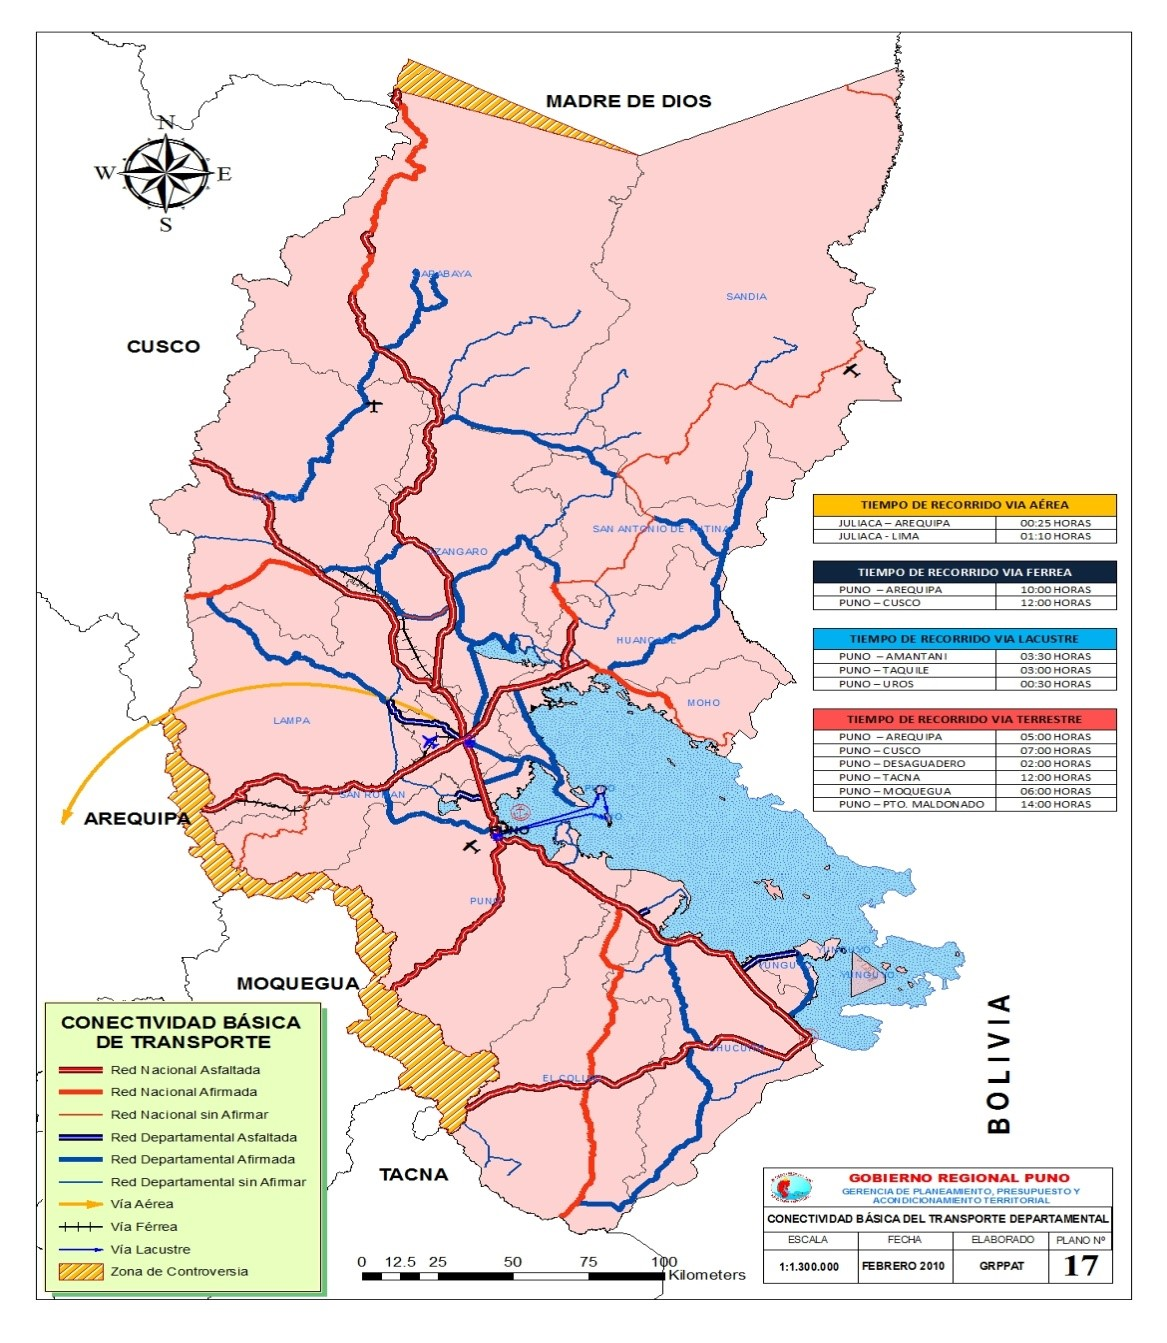
\includegraphics[scale=1]{Capitulo4/Figs/mapa-vial-puno.jpg}
    \caption{Mapa vial de la región Puno}
    Fuente: \citeA{2011PlanPERTUR}
    \label{fig:mapa_vial_puno}
\end{figure}
\subsubsection{Accesibilidad aérea}
"Existen dos lineas aereas que hacen el servicio de pasajeros y carga desde Lima; LAN PERU, y STAR PERU, y a traves de las principales ciudades de la macro region; Cusco, Arequipa y Tacna, hasta y desde la ciudad de Juliaca. El transporte aéreo moviliza el 2.60\% de pasajeros y el 2.82\% en la región.

En la región existen dos pistas de aterrizaje autorizadas; El aeropuerto Inca Manco Capac de la Ciudad de Juliaca, y el aeródromo de la Compañía minera MINSUR – Mina San Rafael ubicado en el distrito de Antauta de la Provincia de Melgar" \cite{2011PlanPERTUR}
\subsubsection{Accesibilidad férrea}
"La rapidez y seguridad que ofrece el transporte terrestre de pasajeros, ha desplazado al tren como medio de transporte de pasajeros. El ferrocarril del sur del Perú, como vía de comunicación es el más extenso que se ha construido y que aún funciona, conecta Puno con Arequipa y Cusco, en los últimos años ha decaído su importancia, aunque continúa operando y brindando servicios de carga y pasajeros, moviliza el 17.54\% de pasajeros y 14.68\% de los volúmenes de carga. La empresa Perú Rail ha privilegiado atender el transporte turístico de pasajeros en la ruta Puno – Juliaca - Cusco - Machu Picchu, con frecuencia diaria a las 8:00 am.. Solo se transporta carga entre las ciudades de Puno Arequipa. La longitud ferroviaria del sur alcanza a 992 kms, une Puno, Juliaca, Arequipa y Matarani, Cusco y Quillabamba. La línea Puno - Arequipa con 351 kms., y la línea Juliaca - Cusco con 338 kms." \cite{2011PlanPERTUR}
\subsubsection{Accesibilidad lacustre}
"Por este medio se moviliza aproximadamente el 3.94\% de pasajeros de la región, el transporte de carga se circunscribe al traslado de productos de primera necesidad, productos artesanales y pesca." \cite{2011PlanPERTUR}
Se tiene  como principales embarcaderos a Puerto de Puno, Barco en Chucuito, Lampayuni en la Isla Amantani y Salacancha y Chilcano en la Isla Taquile.
\subsection{Análisis de la oferta turística}
\subsubsection{Recursos y atractivos turísticos de la Región Puno}
...
Se tiene un inventario de los recursos turísticos de la Región Puno, en el Inventario de Recursos Turísticos a nivel nacional, disponibles en la Pág. Web del MINCETUR. http://sigmincetur.mincetur.gob.pe
\subsubsection{Servicios turísticos de la Región Puno}
\paragraph{Establecimientos de hospedaje-----------------------}
A nivel regional a Diciembre del 2010, se tiene 262 establecimientos de hospedaje, de los cuales 166 establecimientos se encuentran en la provincia de Puno, 64 en San Román y 32 en las provincias de Chucuito, El Collao, Yunguyo, Melgar, Huancané, Moho y Carabaya; del total de los establecimientos 73 son categorizados y 189 no categorizados. Los establecimientos que se encuentran en la provincia de Puno son; un hotel de 5 estrellas, 6 hoteles de 4 estrellas,15 hoteles de 3 estrellas, 8 hoteles de 2 estrellas, 1 hotel de una estrella, 5 hostales de 3 estrellas, 15 hostales de 2 estrellas y 4 hostales de 1 estrella y 1 albergue
\paragraph{Restaurantes}
\paragraph{Agencias de viaje y turismo}
\paragraph{Transporte}
\subsection{Análisis de la demanda turística}



\section{Materiales e insumos}
Técnicas de investigación, instrumentos(materiales)

\section{Metodología}
\subsection{Tipo de investigación}
Esquema
Aplicativas
Teoria+Hecho+Solucion=Propositiva
\subsection{Arquitectura de la solución}
\subsection{Metodología de la investigación}

\chapter{V. ADMINISTRACIÓN DEL PROYECTO DE INVESTIGACIÓN }
\section{Cronograma del proyecto}
...
\section{Presupuesto}
...
\bibliographystyle{apacite}
\renewcommand\bibname{LISTA DE REFERENCIAS}
\bibliography{mendeley}
% documentacion oficial
% http://ctan.dcc.uchile.cl/biblio/bibtex/contrib/apacite/apacite.pdf
\chapter{VII. ANEXOS}
\section{MAPIC}
...

\end{document}